\documentclass[a4paper,12pt]{article}
\usepackage[utf8]{inputenc}
%\usepackage[spanish]{babel}
\usepackage[es]{babel}
\usepackage{geometry}
\usepackage{graphicx}
\usepackage{ragged2e}
\geometry{a4paper, margin=1in}
\begin{document}
\justifying

% Carátula
\begin{titlepage}
    \centering
    % Escudo ESPE
    
\includegraphics[width=0.8\textwidth]{imgs/ESPEtransparente-3766697184.png}\\[1.5cm]
    {\Large Universidad de las Fuerzas Armadas ``ESPE''}\\[1.5cm]
    {\LARGE Aplicaciones Distribuidas}\\[2cm]
    {\large Estudiante: Leonardo Narváez}\\[0.5cm]
    {\large Docente: Geovany Cudco}\\[0.5cm]
    {\large 29/05/2026}\\[3cm]
    {\Huge Resumen}\\[0.5cm]
    \vfill
\end{titlepage}

% --- Resumen fundamentado tipo cuaderno (palabras clave en negrita, conceptos separados, formato mejorado) ---

\section*{Unidad I: Fundamentos de Aplicaciones Distribuidas}

\subsection*{1. Introducción}
Las \textbf{aplicaciones distribuidas} son sistemas cuyo software se ejecuta en múltiples máquinas interconectadas por una red, cooperando para ofrecer una funcionalidad unificada. Son esenciales para la informática moderna, permitiendo \textbf{escalabilidad}, \textbf{tolerancia a fallos} y \textbf{flexibilidad}.

\subsection*{1.1 Conceptos de Aplicaciones Distribuidas}
\begin{description}
    \item[\textbf{Sistema:}] Conjunto de elementos interrelacionados que funcionan como un todo organizado para alcanzar un objetivo común. Puede ser físico, biológico, social o informático. Un sistema informático incluye \textbf{hardware}, \textbf{software}, \textbf{procesos} y \textbf{personas} que interactúan para cumplir objetivos comunes.
    
    \item[\textbf{Aplicación:}] Programa o conjunto de programas diseñados para realizar tareas específicas que satisfacen necesidades concretas de usuarios o negocios. Se apoya en el sistema (hardware, OS y middleware) para ejecutar la lógica de negocio, presentar interfaces al usuario y acceder a datos. Suele componerse de módulos o servicios (backend, frontend, base de datos) que colaboran entre sí.
    \begin{figure}[h!]
        \centering
        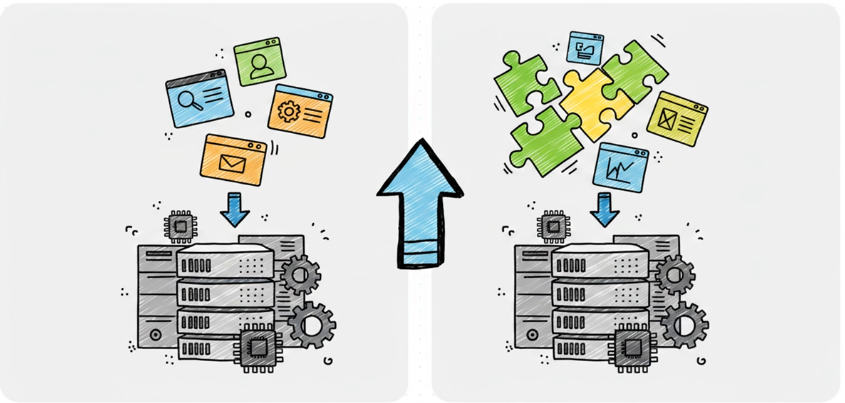
\includegraphics[width=0.8\textwidth]{imgs/Sistema vs Aplicacion.png}
        \caption{Comparación entre Sistema y Aplicación}
        \label{fig:sistema-vs-aplicacion}
    \end{figure}
    \item[\textbf{Distribución:}] Técnica de dividir componentes de un sistema o aplicación en varias ubicaciones físicas o lógicas, normalmente en diferentes máquinas conectadas en red, trabajando juntas para lograr un objetivo común.
    
    \item[\textbf{Sistema Distribuido:}] Conjunto de computadoras independientes que se presentan a los usuarios como un sistema único y coherente, colaborando mediante una red para compartir recursos, procesamiento y almacenamiento.
    
    \item[\textit{Tanenbaum:}] "Un sistema distribuido es una colección de computadoras independientes que aparecen ante los usuarios como una única computadora".
    
    \item[\textit{Coulouris:}] "Los sistemas distribuidos son aquellos en los cuales los componentes de hardware y software están ubicados en computadoras de una red y se comunican y coordinan sus acciones solamente por medio de mensajes".
\end{description}

\subsection*{1.2 Evolución de las Aplicaciones Distribuidas}
\begin{itemize}
    \item \textbf{Décadas 1960–1970:} Se desarrollan los primeros sistemas operativos multiusuario y multitarea como CTSS (MIT, 1961) y UNIX (AT\&T Bell Labs, 1969). Surge la necesidad de compartir recursos computacionales entre usuarios remotos. En 1969 se crea \textbf{ARPANET}, la precursora de Internet, permitiendo la interconexión de computadoras a gran escala. En 1972 se desarrolla el \textbf{correo electrónico} en ARPANET, considerada la primera aplicación distribuida a gran escala.
    
    \item \textbf{Década 1980:} Surgen las \textbf{redes de área local (LAN)} como Ethernet, permitiendo la conexión de computadoras dentro de una misma organización. Se consolida el modelo \textbf{cliente-servidor} como arquitectura estándar para aplicaciones distribuidas. En 1982 se celebra la primera conferencia académica especializada: Symposium on Principles of Distributed Computing (PODC). En 1985 inicia el proyecto ANSA, uno de los primeros intentos por crear una arquitectura de objetos distribuidos. En 1989 se funda el Object Management Group (OMG), que más tarde desarrollará CORBA.
    
    \item \textbf{Década 1990:} En 1990 se publica la primera especificación de \textbf{CORBA} (Common Object Request Broker Architecture), un estándar para objetos distribuidos multiplataforma. En 1992 aparecen las primeras implementaciones comerciales de CORBA. En 1993 se introduce \textbf{CGI} (Common Gateway Interface), permitiendo la creación de páginas web dinámicas y la interacción entre aplicaciones web y servidores. En 1995 Java introduce \textbf{RMI} (Remote Method Invocation), permitiendo la invocación de métodos entre objetos Java en diferentes máquinas. En 1999 se popularizan las aplicaciones cliente-servidor en entornos empresariales, con herramientas como \textbf{DCOM} (Microsoft) y CORBA en diversas industrias.
    
    \item \textbf{Década 2000:} En 2000 Roy Fielding introduce \textbf{REST} (Representational State Transfer), sentando las bases para los servicios web modernos. Entre 2001 y 2003 se consolida \textbf{SOAP} (Simple Object Access Protocol) como estándar para servicios web basados en XML. En 2005 se populariza la \textbf{Arquitectura Orientada a Servicios (SOA)}, promoviendo la reutilización de servicios distribuidos. En 2007 surgen las primeras plataformas de computación en la nube, como \textbf{Google App Engine} (2008).
    
    \item \textbf{Década 2010:} En 2013 se presenta \textbf{Docker}, revolucionando la forma de empaquetar y desplegar aplicaciones distribuidas con contenedores. En 2014 Amazon lanza \textbf{AWS Lambda}, marcando el inicio de la computación serverless. En 2015 se lanza \textbf{Kubernetes}, una plataforma de orquestación de contenedores que se convierte en estándar para aplicaciones distribuidas en la nube. En 2016 Google y Microsoft lanzan \textbf{Google Cloud Functions} y \textbf{Azure Functions}, consolidando el modelo serverless. En 2017 se consolida la arquitectura de \textbf{microservicios} como enfoque dominante para aplicaciones empresariales distribuidas.
    
    \item \textbf{Década 2020:} Se populariza el concepto de \textbf{aplicaciones nativas de la nube (cloud-native)}, combinando microservicios, contenedores, Kubernetes y DevOps. Entre 2021 y 2025 se adoptan ampliamente plataformas serverless y arquitecturas event-driven. Se integran tecnologías como \textbf{mallas de servicio (Service Mesh)} e infraestructura inmutable. Se promueve la automatización total del ciclo de vida de aplicaciones distribuidas con \textbf{GitOps}, \textbf{CI/CD} y \textbf{observabilidad avanzada}.
\end{itemize}

\subsection*{1.3 Principales Desafíos y Ventajas}
\textbf{Ventajas:}
\begin{itemize}
    \item Escalabilidad horizontal: Permite añadir más nodos (servidores, contenedores, dispositivos) para manejar mayor carga, en lugar de depender de hardware más potente. Esto es clave en entornos cloud y para aplicaciones con tráfico variable.
    \item Alta disponibilidad y tolerancia a fallos: Al distribuir la carga y replicar servicios en múltiples nodos o regiones, el sistema puede seguir funcionando aunque uno o varios componentes fallen. Esto se logra mediante redundancia y patrones como el “disyuntor” (circuit breaker).
    \item Mejor rendimiento mediante procesamiento paralelo: Las tareas complejas pueden dividirse y ejecutarse simultáneamente en distintos nodos, acelerando su resolución (ejemplo: análisis de big data con Spark, IA distribuida).
    \item Compartición eficiente de recursos: Permite el uso compartido de hardware costoso (almacenamiento, GPUs, impresoras) y datos entre múltiples usuarios o sistemas, optimizando costos y acceso.
    \item Flexibilidad tecnológica: Cada componente (microservicio, nodo) puede usar la tecnología más adecuada para su función (lenguaje, base de datos, framework), facilitando la innovación y el mantenimiento.
\end{itemize}
\textbf{Desventajas:}
\begin{itemize}
    \item Mayor complejidad de desarrollo y mantenimiento: Coordinar múltiples servicios, gestionar la comunicación asíncrona, depurar fallos distribuidos y manejar versiones compatibles requiere herramientas y conocimientos avanzados.
    \item Costos operativos más altos: Aunque el hardware puede ser más económico, los costos de red, monitoreo, orquestación (Kubernetes), seguridad y personal especializado suelen ser significativos.
    \item Sobrecarga de red y procesamiento: La comunicación constante entre nodos consume ancho de banda, CPU y memoria. Protocolos, serialización, autenticación y reintentos añaden latencia y consumo innecesario si no se optimizan.
    \item Superficie de ataque ampliada: Cada nodo, API o conexión es un posible punto de entrada para atacantes. La seguridad debe implementarse en múltiples capas (red, aplicación, datos), lo que es más difícil que en sistemas centralizados.
    \item Dificultad para garantizar la coherencia fuerte: Mantener todos los datos sincronizados en tiempo real entre nodos es costoso y a menudo inviable. Muchos sistemas optan por coherencia eventual, lo que puede generar inconsistencias temporales.
\end{itemize}
\textbf{Desafíos:}
\begin{itemize}
    \item Gestión de la latencia de red: La comunicación entre nodos introduce retrasos impredecibles, afectando la experiencia del usuario y la lógica de negocio, especialmente en llamadas encadenadas (problema del “chatty API”).
    \item Observabilidad y monitoreo integral: Es difícil rastrear una transacción que atraviesa decenas de servicios. Se requieren herramientas avanzadas de logging, métricas y trazado distribuido (como OpenTelemetry) para diagnosticar problemas.
    \item Coordinación de transacciones distribuidas: Las transacciones ACID tradicionales no se aplican fácilmente. Se deben usar patrones alternativos como Saga, transacciones compensatorias o CQRS, que son más complejos de implementar.
    \item Gestión de la heterogeneidad: Integrar dispositivos, protocolos, lenguajes y sistemas operativos diversos (especialmente en IoT o edge) requiere estándares abiertos y middleware robusto para garantizar interoperabilidad.
    \item Actualización y despliegue continuo seguro: Desplegar cambios en cientos de microservicios sin interrumpir el servicio exige estrategias como canary releases, blue-green deployments y pruebas automatizadas exhaustivas.
\end{itemize}

\subsection*{1.4 Falacias de las Aplicaciones Distribuidas}
Son una lista clásica de suposiciones erróneas que los desarrolladores suelen hacer al diseñar aplicaciones distribuidas. Fueron formuladas originalmente por L. Peter Deutsch y otros ingenieros de Sun Microsystems en la década de 1990. Siguen siendo profundamente relevantes hoy en día, especialmente con la proliferación de microservicios, nube, IoT y edge computing.
\begin{enumerate}
    \item \textbf{La red es fiable:} Las redes fallan constantemente: cortes de fibra, errores de hardware, congestión, problemas de ISP, etc. Aplicaciones que no manejan reintentos, timeouts o caídas de red se bloquean o pierden datos. Ejemplo: una llamada a un microservicio sin manejo de errores puede colapsar todo el flujo.
    \item \textbf{La latencia es cero:} La comunicación a través de la red siempre tiene retraso (latencia), que varía según la distancia, congestión y protocolo. Diseños que asumen respuestas instantáneas generan interfaces lentas, timeouts y mala experiencia de usuario.
    \item \textbf{El ancho de banda es infinito:} El ancho de banda es limitado y compartido. Transferir grandes volúmenes de datos sin compresión o paginación satura la red, ralentiza otros servicios y aumenta costos.
    \item \textbf{La red es segura:} Las redes, especialmente las públicas o inalámbricas, están expuestas a sniffing, MITM, DDoS, inyecciones, etc. Transmitir datos sin cifrado, usar credenciales débiles o confiar ciegamente en la red expone información sensible y permite ataques.
    \item \textbf{La topología de la red no cambia:} Los nodos se mueven, se agregan o eliminan, y las rutas de red cambian constantemente. Aplicaciones que almacenan direcciones IP fijas o asumen rutas estáticas fallan al migrar a la nube o usar contenedores.
    \item \textbf{Hay un solo administrador de la red:} En entornos modernos, múltiples equipos, proveedores y organizaciones gestionan partes de la infraestructura. Falta de coordinación lleva a brechas operativas, conflictos de IP o problemas de cumplimiento normativo.
    \item \textbf{El costo del transporte es cero:} Cada byte transmitido tiene un costo monetario, energético y de rendimiento. Arquitecturas "chatty" o transferencias innecesarias elevan facturas de nube, agotan baterías y saturan CPUs.
    \item \textbf{La red es homogénea:} Coexisten múltiples protocolos, sistemas operativos, lenguajes, firewalls, NATs, proxies y dispositivos con capacidades distintas. Suponer que todos los nodos se comunican igual causa fallos de interoperabilidad.
\end{enumerate}

\subsection*{1.5 Teorema CAP}
El teorema CAP, propuesto por Eric Brewer en el año 2000, define el comportamiento de un sistema distribuido. Está formado por la primera letra de cada atributo: Consistency (Consistencia), Availability (Disponibilidad) y Partition tolerance (Tolerancia a particiones). Un sistema distribuido es un grupo de nodos conectados que comparten información entre sí. Un cliente puede escribir un dato interactuando con cualquier nodo y puede leerlo del mismo nodo o de uno diferente. El teorema establece que, para una operación de escritura seguida de una lectura, el sistema solo puede garantizar dos de tres atributos simultáneamente, debiendo sacrificar el tercero. En la computación distribuida la red nunca es confiable, por lo tanto, se debe escoger entre mantener la consistencia o la accesibilidad.
\begin{itemize}
    \item \textbf{Consistencia:} Todos los nodos ven los mismos datos al mismo tiempo, garantiza que no se devuelva data desactualizada.
    \item \textbf{Disponibilidad:} Si un nodo se encuentra abajo, el sistema tiene que responder a las peticiones enviadas. Un nodo activo debe devolver una respuesta razonable en un periodo de tiempo razonable.
    \item \textbf{Tolerancia a particiones:} Un sistema debe seguir funcionando aun cuando los nodos no se puedan comunicar entre sí (temporal o permanentemente).
\end{itemize}

\subsection*{1.6 Gestión de Concurrencia}
La concurrencia permite manejar múltiples tareas simultáneamente en nodos remotos. Mejora el rendimiento y la escalabilidad en entornos como la nube o microservicios. Sin embargo, introduce desafíos únicos: latencia de red, fallos parciales y problemas de consistencia de datos. La concurrencia distribuida crea una ilusión de simultaneidad entre nodos que no ejecutan en paralelo real. Se basa en comunicación asíncrona, como HTTP o mensajería. Los problemas comunes incluyen condiciones de carrera, donde dos nodos modifican el mismo recurso al mismo tiempo, generando inconsistencias. Otros riesgos son deadlocks, que bloquean procesos mutuamente, y starvation, donde tareas se ignoran indefinidamente. En bases de datos como Cassandra, se elige consistencia eventual sobre fuerte para priorizar disponibilidad. Paradigmas para manejar concurrencia incluyen el modelo de Actores (como Akka), que encapsula estado en actores que se comunican por mensajes inmutables, evitando compartición directa, y el modelo de Flujos Reactivos (como RxJava), que gestiona streams de datos asíncronos para procesar eventos en tiempo real.

\subsection*{1.7 Hilos de Ejecución en Programación Distribuida}
Los hilos son unidades básicas de concurrencia, pero en sistemas distribuidos suelen pausar para esperar respuestas remotas, agregando overhead de red. En Java o Go, se crean con Thread o goroutines, integrados en pools para escalabilidad horizontal. Frameworks como Kubernetes orquestan contenedores con pools de hilos distribuidos.

\subsection*{Resumen Final}
Las aplicaciones distribuidas son la base de los sistemas modernos, permitiendo colaboración entre múltiples nodos para ofrecer servicios escalables, tolerantes a fallos y flexibles. Comprender su evolución, ventajas, desafíos y buenas prácticas es esencial para diseñar soluciones robustas y eficientes.

\end{document}
